\documentclass[notitlepage]{beamer}
\usepackage[utf8]{inputenc}
\usepackage[catalan]{babel}
\usepackage{url}

%%%%%% Per realitzar diagrames de fluxe %%%%%%

\usepackage{tikz}
\usetikzlibrary{arrows,shadows}
\usepackage{pgf-umlsd} 

%\setbeameroption{show notes on second screen=right}
\setbeamertemplate{navigation symbols}{} 

%\usetheme[secheader]{Boadilla}
\usetheme{Copenhagen}
%\usetheme{Darmstadt}
%\usetheme{Frankfurt}
%\usetheme{Goettingen}
%\usetheme{Hannover}
%\usetheme{Luebeck}
%\usetheme[secheader]{Madrid}
%\usetheme{Warsaw}


\hypersetup{pdfpagemode=FullScreen}

\title[Implementació de la botifarra a través de Web]{Implementació de la Botifarra amb WebSockets, HTML5 i Javascript }
\subtitle{Treball de Final de Màster\\Universitat de Lleida\\Escola Politècnica Superiror}
\author{Sergi Almacellas Abellana pokoli@gmail.com}
\date{\today}

\setbeamercovered{transparent}

\begin{document}


\begin{frame}
\begin{center} 

\Large Màster en Enginyeria de Programari Lliure\\
\textsc{\LARGE Treball de Final de Màster}\\[0.5cm]


{\huge \bf Implementació de la Botifarra utilitzant WebSocket, HTML5 i Javascript } \\[0.75cm]

\textsl{Autor: Sergi Almacellas Abellana}\\
\textsl{Director: Juan Manuel Gimeno Illa}\\ 

\vfill{26 de juliol de 2012}
\end{center}
\end{frame}

\begin{frame}
\tableofcontents
\end{frame}

\section{Introducció}
\begin{frame}
\frametitle{Introducció}
\begin{block}{Què és la botifarra?}
\begin{itemize}
    \item{Joc de Cartes, que utilitza la baralla espanyola.}
    \item{Tradicionalment jugat a Catalunya.}
    \item{4 Jugadors, 2 equips de 2 jugadors.}
\end{itemize}
\end{block}

\begin{block}{Què s'ha implementat?}
El joc de la botifarra a través de navegador web.
\end{block}
\end{frame}


\subsection{Objectius}
\begin{frame}
\frametitle{Objectius}
\begin{block}{Objectius principals}
\begin{itemize}
    \item{Implementar un joc de la botifarra.}
    \item{Presa de contacte amb noves tecnologies.}  
\end{itemize}
\end{block}

\begin{block}{Objectius secundaris}
\begin{itemize}
    \item{Utilitzar forges per la compartició de codi.}
    \item{Utilitzar noves metodologies de treball ( TDD/BDD)}  
\end{itemize}
\end{block}

\end{frame}


\subsection{Requeriments del sistema}
\begin{frame}
\frametitle{Requeriments del sistema}
\begin{block}{Lògica Botifarra}
\begin{itemize}
    \item{Complir amb les regles de la botifarra.}
    \item{Jugadors automatitzats.}
\end{itemize}
\end{block}

\begin{block}{Entorn Web}
\begin{itemize}
    \item{Programa servidor}
    \item{Programa client}
\end{itemize}
\end{block}

\begin{block}{Multijugador}
\begin{itemize}
    \item{Permetre comunicació entre els jugadors.}
    \item{Temps real.}
    \item{Capaç d'allotjar gran quantitat de jugadors.}
\end{itemize}
\end{block}
\end{frame}

\section{Metodologia}
\begin{frame}
\frametitle{Metodologia}
\begin{block}{Metodologies Utilitzades}
    \begin{enumerate}
    \item{Model Incremental}
    \item{TDD/BDD}
    \end{enumerate}
\end{block}
\begin{block}{TDD/BDD}
    \begin{enumerate}
    \item{Definir la característica a implementar.}
    \item{Escriure la seva especificació.}
    \item{Escriure la implementació.}
    \item{Comprovar la validesa de la implementació.}
    \item{Reestructurar/millorar la implementació.}
    \end{enumerate}
\end{block}
\end{frame}

\section{Tecnologies utilitzades}
\begin{frame}
\frametitle{Tecnologies utilitzades}
\begin{block}{Principals}
    \begin{enumerate}
    \item{Node.js}
    \item{WebSockets}
    \item{HTML5}
    \end{enumerate}
\end{block}
\begin{block}{Altres}
    \begin{enumerate}
    \item{JQuery, CSS i Jade}
    \item{JSON}
    \item{Mocha i JsCoverage}
    \item{Git}
    \end{enumerate}
\end{block}
\end{frame}

\subsection{Node.js}
\begin{frame}
\frametitle{Node.js}
\begin{block}{Què es Node.js}
Framework multiplataforma execució codi Javascript per la banda del servidor.
\end{block}

\begin{block}{Característiques}
\begin{itemize}
    \item{Entrada/Sortida Asíncrona.}
    \item{Múltiples fils d'execució de forma transparent per al programador.}
    \item{Basat en esdeveniments.}
    \item{Gran quantitat de llibreries disponibles i gestor de les mateixes.}
    \item{Suport integrat pels protocols TCP,DNS,HTTP.}
\end{itemize}
\end{block}

\end{frame}

\begin{frame}
\frametitle{Codi síncron vs. codi asíncron}
\begin{block}{Códi síncron:}
Espera a obtenir els recursos externs (Fitxers,BD). Necessitat d'us dels threads per paralelitzar.
\end{block}

\begin{block}{Codi asíncron:}
NO s'espera, es programa l'execució de codi quan el recurs estigui disponible.
\end{block}

\begin{block}{Com s'implementa en node?}
\begin{itemize}
    \item{Bucle d'esdeveniments.}
    \item{Emisió d'events.}
\end{itemize}
\end{block}

\end{frame}

\begin{frame}
\frametitle{Node.js}
\begin{block}{Beneficis de Node.js}
\begin{itemize}
    \item{No hi ha bloquejos.}
    \item{Simplicitat del codi.}
    \item{Velocitat.}
\end{itemize}
\end{block}
\begin{block}{Per a què s'utilitza?}
\begin{itemize}
    \item{Desenvolupament d'aplicacions o serveis web.}
    \item{Sistemes d'intercanvi de missatges.}
    \item{Servidors per a jocs multijugador basats en HTML5}
\end{itemize}
\end{block}

\end{frame}

\subsection{WebSockets}
\begin{frame}
\frametitle{WebSockets}
\begin{block}{Problemes del protocol HTTP}
\begin{itemize}
    \item{Comunicació unidireccional.}
    \item{Gran quantitat d'informació addicional (capçaleres).}
    \item{Refresc de la informació.}
\end{itemize}
\end{block}

\begin{block}{Que ens permeten els WebSockets?}
\begin{itemize}
   \item{Canal de comunicació bidireccional.}
    \item{Reduir la informació addicional.}
    \item{Informació en temps real.}
\end{itemize}
\end{block}
\end{frame}

\subsection{HTML5}
\begin{frame}
\frametitle{HTML5}
\begin{block}{Què és HTML5?}
Última versió del llenguatge de marcatge utilitzat per escriure pàgines web.
\end{block}

\begin{block}{Novetats}
\begin{enumerate}
    \item{Millor estructuració del documents.}
    \item{Contingut multimèdia: àudio, vídeo, animacions (canvas).}
\end{enumerate}
\end{block}

\begin{block}{Beneficis}
A l'estar estandarditzats són suportats de forma nativa per tots els navegadors web moderns.
\end{block}
\end{frame}


\subsection{Per a què s'utilitzen?}
\begin{frame}
\frametitle{Per a què s'utilitzen?}
\begin{block}{Node.js}
Encarregat d'allotjar tota la lògica del servidor de partides.
\end{block}

\begin{block}{Websockets}
S'encarrega de realitzar el transport de la informació entre el client i el servidor.
\end{block}

\begin{block}{HTML5}
S'utilitza l'etiqueta canvas per tal de dibuixar la interfície del joc i realitzar les animacions corresponents
\end{block}
\end{frame}

\begin{frame}
\frametitle{Per a què s'utilitzen?}
\begin{block}{Altres}
\begin{itemize}
    \item{jQuery, CSS, Jade $\Rightarrow$  Capa de presentació del sistema.}
    \item{JSON $\Rightarrow$  Estructuració de la informació que s'envia a través dels WebSockets.}
    \item{Mocha i JSCoverage $\Rightarrow$ Jocs de Proves}
    \item{Git $\Rightarrow$  Allotjament del codi font}

\end{itemize}
\end{block}
\end{frame}

\section{Desenvolupament}
\subsection{Lògica Botifarra}
\begin{frame}
\frametitle{Lògica Botifarra}
\centering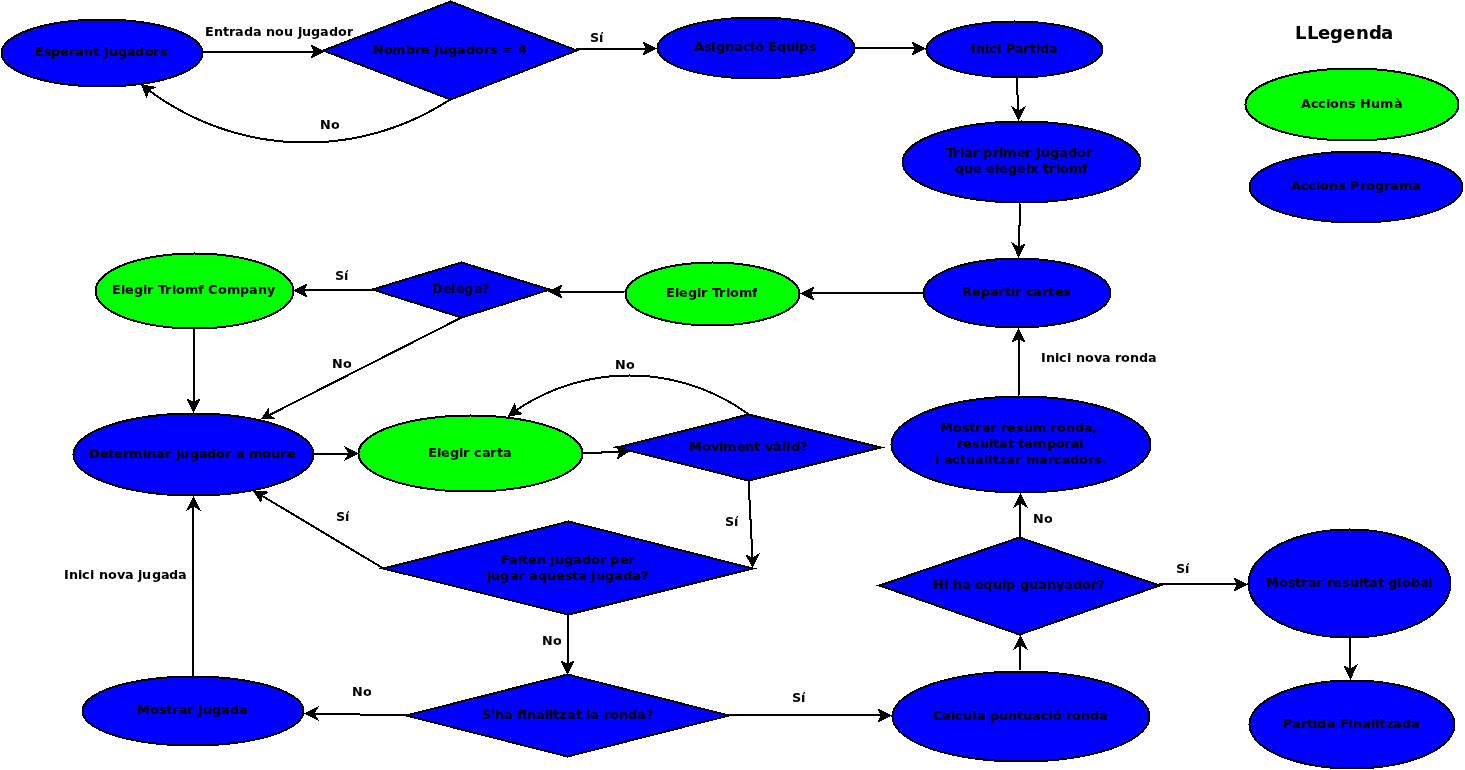
\includegraphics[width=10cm]{img/butifarra_workflow.png}
\end{frame}

\subsection{Comunicació client-servidor}
\begin{frame}
\centering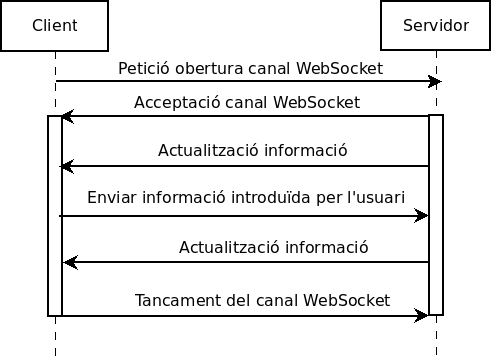
\includegraphics[width=10cm]{img/diagrama-websocket.png}
\end{frame}

\section{Demostració}
\begin{frame}
\frametitle{Provem-ho}
\begin{center}
\url{http://buti.koolpi.com}
\end{center}
\end{frame}

\section{Conclusions}
\begin{frame}
\frametitle{Conclusions}
\begin{block}{TDD/BDD}
\begin{itemize}
\item{Augmenten l'estabilitat del codi $\Rightarrow$ millora de la productivitat.}
\item{Permet mesurar l'estat del desenvolupament.}
\end{itemize}
\end{block}

\begin{block}{HTML5}
\begin{itemize}
\item{Augment de característiques $\Rightarrow$ semblança entorn d'escriptori.}
\end{itemize}
\end{block}

\begin{block}{WebSockets}
\begin{itemize}
\item{Gran volum de dades  $\Rightarrow$ millora el real-time.}
\end{itemize}
\end{block}

\begin{block}{Node.js}
\begin{itemize}
\item{Estabilitat + Conjunt de mòduls $\Rightarrow$ facilitat desenvolupament.}
\item{Disseny asíncron + Esdeveniments $\Rightarrow$ + peticions - recursos.}
\end{itemize}
\end{block}
\end{frame}


\begin{frame}
\frametitle{Conclusions}
\begin{block}{Desenvolupament d'aplicacions web.}
\begin{itemize}
\item{Independència Sistema Operatiu.}
\item{Independència Tipus dispositiu.}
\item{Sense realitzar cap tipus d'instal·lació.}
\item{Permet la compartició d'informació.}
\end{itemize}
\end{block}

\begin{block}{Què suposa?}
Gran futur en el desenvolupament d'aplicacions.
\end{block}
\end{frame}

\begin{frame}
\frametitle{Treball futur}
\begin{itemize}
\item{Adaptació interfície telèfons mòbils.}
\item{Histrrial de partides.}
\item{Classificació de jugadors.}
\item{Millora de la inteligència aritifical.}
\item{Implementació variants de la botifarra.}
\item{Implementació de campionats.}
\item{Integració amb xarxes socials.}
\end{itemize}
\end{frame}


\begin{frame}
\begin{block}{Voleu col·laborar amb el projecte?}
\url{https://github.com/pokoli/ButiJS}
\end{block}

\begin{block}{Dubtes/Preguntes?}
\begin{description}
\item[Correu electrònic:]{pokoli@gmail.com}
\item[Twitter:]{@pokoli\_srk}
\end{description}
\end{block}

\end{frame}
\end{document}
